\documentclass[a4paper, 12pt]{article}

\def \srcdir{tex/}
\def \picdir{pic/}

\input{\srcdir properties}
\input{\srcdir macros}

\title{
  Лабораторная работа \textnumero \input{\srcdir index}\\
  \textbf{\textquote{\input{\srcdir name}\unskip}}
}
\author{\input{\srcdir author}}
\date{\input{\srcdir date}}

\begin{document}

\maketitle\thispagestyle{fancy}

\subsection*{Цель работы}
Измерить коэффициент теплопроводности воздуха при атмосферном\
давлении в зависимости от температуры.

\subsection*{Оборудование}
\begin{itemize}[noitemsep]
  \item Цилиндрическая колба с натянутой по оси нитью
  \item Термостат
  \item Вольтметр и амперметр (цифровые мультиметры)
  \item Эталонное сопротивление
  \item Источник постоянного напряжения
  \item Реостат (или магазин сопротивлений)
\end{itemize}

\subsection*{{Ход работы}}
\subsubsection*{\Rnum{1}. Теоретическая справка}

Рассмотрим стационарную теплопроводность в цилиндрической геометрии (см. \textbf{рис. \ref{fig:1}}).\
Пусть тонкая нить радиусом $r_1$ и длиной $L$ помещена на оси цилиндра радиусом $r_0$.\
Температура стенок цилиндра $T_0$ поддерживается постоянной. Пусть в нити выделяется\
некоторая тепловая мощность $Q$ [Вт]. Если цилиндр длинный $(L \gg r_0)$, можно пренебречь\
теплоотводом через его торцы. Тогда все параметры газа можно считать зависящими только\
от расстояния до оси системы $r$, а поток тепла $\vec{q}$ направленным строго радиально.\
Закон Фурье для нашей системы имеет вид
\begin{equation}
  q = -\kappa \frac{\mathrm{d}^{} T}{\mathrm{d} r^{}}.
\end{equation}
В стационарном состоянии полный поток тепла через любую цилиндрическую поверхность\
радиуса $r$ площадью $S = 2 \pi rL$ должен быть одинаков и равен $Q = qS$:
\begin{equation} \label{eq:2}
  Q = -2 \pi r L \cdot \kappa \frac{\mathrm{d}^{} T}{\mathrm{d} r^{}} = \text{const}.
\end{equation}
Если перепад температуры $\Delta T = T_1 - T_0$ между нитью и стенками цилиндра мал\
$(\Delta T \ll T_0)$, то в (4) можно пренебречь изменением теплопроводности от температуры\
в пределах системы, положив $\kappa \approx \kappa(T_0)$. Тогда разделяя переменные в \eqref{eq:2} и\
интегрируя от радиуса нити до радиуса колбы, получим
\begin{equation*}
Q = \frac{2 \pi L}{\ln{\sfrac{r_0}{r_1}}}\kappa \Delta T.
\end{equation*}
Похуй?

\subsubsection*{\Rnum{2}. Пиво темное}
\begin{wrapfigure}{R}[0mm]{35mm}
  \caption{Banka piva}\label{fig:1}
  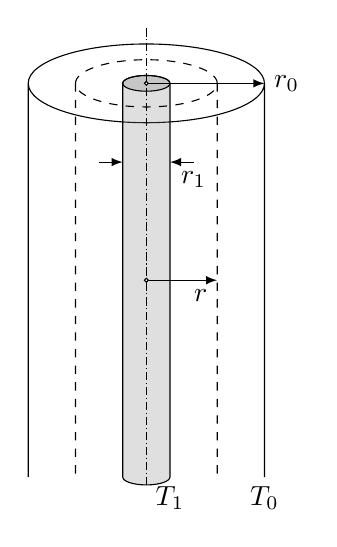
\begin{tikzpicture}[>=latex]
    \coordinate (A) at (10mm,50mm);
    \coordinate (B) at (40mm,50mm);
    \coordinate (C) at (40mm,0);
    \coordinate (D) at (10mm,0);
    \draw
    (A) arc (180:-360:15mm and 5mm)
    (A) -- (D)
    (B) -- (C);
    \node[below] at (C) {$T_0$};

    \coordinate (a) at (22mm,50mm);
    \coordinate (b) at (28mm,50mm);
    \coordinate (c) at (28mm,0);
    \coordinate (d) at (22mm,0);
    \draw [fill=gray, fill opacity=0.25]
    (a) -- (d)
    arc (180:360:3mm and 1mm)
    (c) -- (b)
    arc (0:180:3mm and 1mm);
    \draw [fill=gray, fill opacity=0.25]
    (25mm,50mm) circle (3mm and 1mm);
    \node[below] at (c) {$T_1$};

    \coordinate (a') at (16mm,50mm);
    \coordinate (b') at (34mm,50mm);
    \coordinate (c') at (34mm,0);
    \coordinate (d') at (16mm,0);
    \draw [dashed]
    (a') arc (180:-360:9mm and 3mm)
    (a') -- (d')
    (b') -- (c');

    \draw [densely dashdotted] (25mm,57mm) -- (25mm,-1mm);
    \draw
    (25mm,50mm) node [anchor=center, circle, draw, solid, inner sep=.5pt, fill=white] {}
    edge [->] node [pos=1, right] {$r_0$} +(15mm,0)
    (19mm,40mm) edge [->] +(3mm,0)
    (31mm,40mm) edge [->] node [pos=0, below] {$r_1$} +(-3mm,0)
    (25mm,25mm) node [anchor=center, circle, draw, solid, inner sep=.5pt, fill=white] {}
    edge [->] node [pos=1, below left] {$r$} +(9mm,0);
  \end{tikzpicture}
\end{wrapfigure}
\lipsum[3-5]

\subsubsection*{\Rnum{3}. Пиво \textquote{Невское}}
\lipsum[6-6]

\subsection*{{Вывод}}
\lipsum[7-7]

\end{document}


